% -----------
% SETUP
% -----------
\documentclass{physics_article_B}
\title{Mechanical Vibrations of Droplets in Fluidic Systems}
\mytitle{Mechanical Vibrations of Droplets in Fluidic Systems}
\myname{Oliver Gordon \& Dominic Coy}
\studentid{4224942 \& 4227789}
\date{Due Date: 1 June 2018}

\begin{document}
	
% ----------------------
% COVERSHEET
% ----------------------
\pagenumbering{roman} 
\setcounter{page}{0}
%\includepdf[scale=1]{Images/Cover.pdf}
%\maketitle

% ----------------------
% ABSTRACT
% ----------------------
\pagenumbering{gobble} 
\begin{abstract}
	\large{Stuff
}
\end{abstract}
	
% ----------------------
% CONTENTS
% ----------------------
%\vspace{4cm}

\tableofcontents

\pagenumbering{roman} 
\setcounter{page}{1}
	
% ----------------------
% INTRODUCTION
% ----------------------
\newpage
\pagenumbering{arabic} 
\setcounter{page}{1}

% ----------------------
% Literature Review
% ----------------------
\newpage

\section{Introduction\label{sect:intro}}

\section{Literature Review\label{sect:litrev}}

\section{Theory\label{sect:theory}}

\section{Oscillating Droplets}
    \subsection{Motor Control}
	\subsection{Electric Field}
	\subsection{Distortion}

% ----------------------
% Equipment
% ----------------------
\section{Fluid Circuit\label{sect_loop}}
A user-friendly toolbox was developed in MATLAB to allow these steps to be automated.

\begin{figure}[H]
\centering
\hspace*{-0.9cm}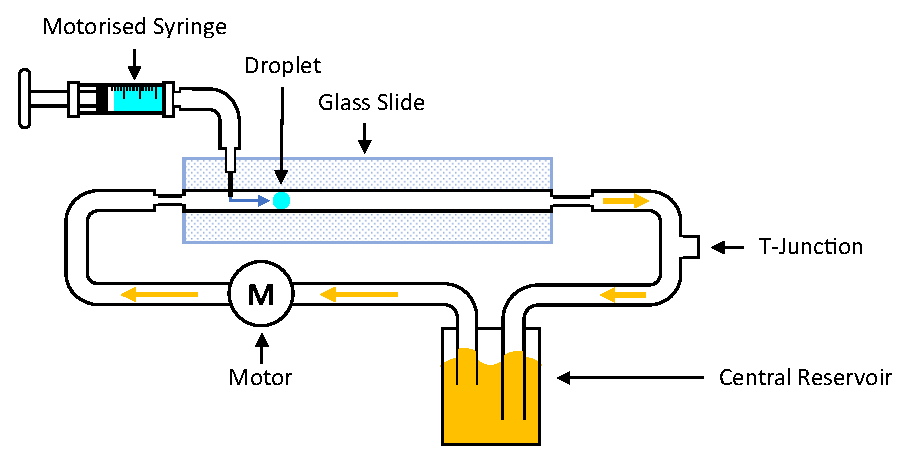
\includegraphics[scale=0.8]{Figures/Fluid.eps}
\captionsetup{justification=centering}
\caption{Words.} 	
\label{fig:basic}
\end{figure} 


\subsection{Motor}
Code was written to automatically interface with the pump over a COM port. This also has a significant delay, reducing the throughput of droplets.\\

Motor also needed to be controlled, as...

\subsection{Creating Droplets}

% ----------------------
% Computer Vision
% ----------------------
\subsection{Computer Vision\label{sect_vision}}
    
    \subsubsection{Acquiring Data}
    In order to allow droplets to be analysed in real time, a computer vision control system was developed. A Logitech C920 camera was chosen for its high image quality, high resolution, and wide field of view. \\
    
    Because droplets are not static, strict requirements are placed on the efficiency of calculations. Further, as MATLAB is an interpreted language and lacks hardware acceleration, webcam acquisition operates at very low framerates, making tracking moving droplets in real time difficult. This was overcome by modifying Hebicam\cite{HebiCam}, which was originally created for streaming CCTV footage, and is a MATLAB wrapper for the more efficient openCV. After adapting this package for use with USB webcams, 1080p video could be acquired at 30FPS with processor overhead to perform calculations, as opposed to <6 with none. Furthermore, data was acquired in grayscale (as opposed to RGB), further increasing capture efficiency and reducing the size of stored data. 
    
    \subsubsection{Calibration}
    
    To ensure that droplets were calculated accurately, the webcam had to be calibrated. 20 images of a 10x11, 0.20mm checkerboard pattern were taken at different positions in similar positions to those used during our experiment, as demonstrated in Figure \ref{fig:calib:pos}. An algorithm implemented in MATLAB\cite{CameraCalib} was then used to calculate various extrinsic properties of the camera, such as the optical centre, distortions, and focal lengths in x and y. As shown in Figure \ref{fig:calib:error}, the extrinsics of the camera were calculated to a sub-pixel accuracy of 0.41 pixels, indicating a high quality calibration which will produce errors of less than the precision of the droplet finding algorithm discussed later. \\
    
    \begin{figure}[H]
        \centering
        \begin{subfigure}[b]{0.4\textwidth}
            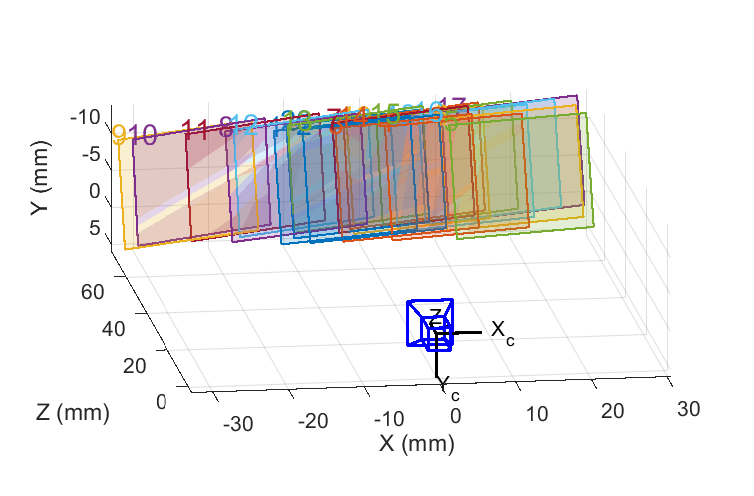
\includegraphics[width=\textwidth]{Figures/CameraExtrinsics.eps}
            \caption{Background}
            \label{fig:calib:pos}
        \end{subfigure}
        \begin{subfigure}[b]{0.4\textwidth}
            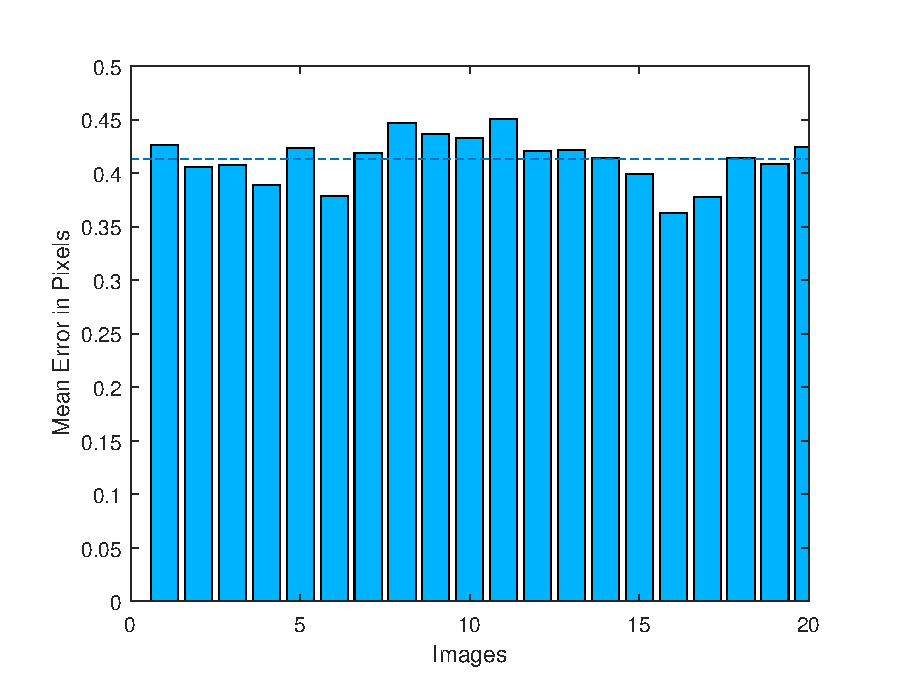
\includegraphics[width=\textwidth]{Figures/CameraError.eps}
            \caption{Foreground}
            \label{fig:calib:error}
        \end{subfigure}
        \caption{Figure }\label{fig:calib}
    \end{figure}
    
    To calculate the size of an object and because a webcam has no depth perception, the checkerboard had to be placed in plane with the droplets. Because the slide was of a finite size, a limitation was placed on the size of the checkerboard. Larger checkers had a lower percentage error from imperfect focusing, yet less of them could be placed on a slide. To determine the optimum size for our purposes, we calibrated the camera with checkers between 1.50 and 5.00mm in size. \\
    
    To determine the optimum checker size, photos containing the checkerboard and circles of radius 0.10 to 1.00mm were taken. A simple circle finding algorithm was then used to find a bounding box around each circle. After correcting the bounding box for fish-eye in the lens, the height and width, $\Delta x$ and $\Delta y$ respectively, of the bounding box was converted from pixels to mm. The radius, $r$, of each circle was then computed with simple trigonometry:
    
    \begin{equation}\label{eq:radii}
        r = \sqrt{\Big(\frac{\Delta x}{2}\Big)^2 + \Big(\frac{\Delta y}{2}\Big)^2}
    \end{equation}
    
    \vspace{3pt} It was found that a 10x11, 0.20mm checkerboard gave the lowest error of 0.03mm. This is shown in Figure \ref{fig:calibsize}. 
    
    \begin{figure}[H]
        \centering
        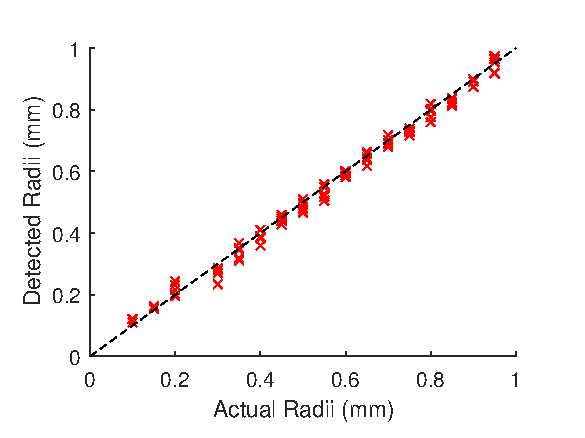
\includegraphics{Figures/CameraCalib.eps}
        \caption{Caption}
        \label{fig:calibsize}
    \end{figure}
    
    From here, it can clearly be seen that the algorithm works as intended (more words)
    
    \subsubsection{Observing}
    To track droplets, a background photograph was first taken with oil flowing but no droplet present. A small 3mm long window along the channel was then defined and continuously monitored. After each frame was captured, this window was subtracted from the corresponding background region, and multiplied by the arbitrarily selected log(6) to act as a gain (thereby increasing contrast). When a droplet was present in the window, this resulted in bright regions where the two images were very different. Once an arbitrary threshold of bright pixels was reached, the droplet was confirmed as being in the window. This algorithm is demonstrated in Figure \ref{fig:detector}. Although this logical test based on bright pixel number is sensitive to noise, it was chosen over an object finder as calculations had to be performed in under 1/30 of a second, as otherwise the droplet could pass the window and fail to be detected, causing the entire system to fail. This noise means that the carrier fluid must be single coloured and free of impurities. \\
    
    \begin{figure}[H]
        \centering
        \begin{subfigure}[b]{0.3\textwidth}
            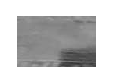
\includegraphics[width=\textwidth]{Figures/DropFinder1.eps}
            \caption{Background}
            \label{fig:detector:back}
        \end{subfigure}
        ~ %add desired spacing between images, e. g. ~, \quad, \qquad, \hfill etc. 
          %(or a blank line to force the subfigure onto a new line)
        \begin{subfigure}[b]{0.3\textwidth}
            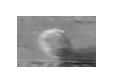
\includegraphics[width=\textwidth]{Figures/DropFinder2.eps}
            \caption{Foreground}
            \label{fig:detector:fore}
        \end{subfigure}
        ~ %add desired spacing between images, e. g. ~, \quad, \qquad, \hfill etc. 
        %(or a blank line to force the subfigure onto a new line)
        \begin{subfigure}[b]{0.3\textwidth}
            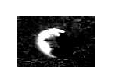
\includegraphics[width=\textwidth]{Figures/DropFinder3.eps}
            \caption{Difference}
            \label{fig:detector:diff}
        \end{subfigure}
        \caption{Figure to demonstrate how droplets are detected after being created by a mechanical pump. A region of the webcam is defined, and a background image taken of this region (a). This region is continuously monitored, and every frame the region is looked at (b), with a comparison made. When enough bright pixels are observed (c), a droplet is considered to be present in the system.}\label{fig:detector}
    \end{figure}
    
    \subsubsection{Determining Droplet Size\label{sect:size}}
    Once a droplet was detected, its outline had to be calculated to later determine its size. Despite the common requirement of the oil industry to identify droplets in a wide range of industries\cite{bubblegeneral}, this is a very difficult task for multiple reasons. For one, without perfect, even lighting surrounding the droplet, droplets do not have bright regions of contrast fully around their boundary. A droplet is also transparent, resulting in the centre looking identical to its surrounding. Droplets can also have bright reflections in their middle, further confusing simple algorithms\cite{bubble1}. The presence of noise in images is also problematic to more sensitive methods. More complex algorithms can take nearly a minute to run\cite{bubble2}, and still only achieve accuracies of approximately 80\%\cite{bubble2}.\\
    
    For our purposes, we begin by stopping the motor and capturing a new image. It was inadequate to use the image previously captured (seen in Figure \ref{fig:detector:fore}) as there was significant motion blur owing to the fact that the droplet was moving. After stopping the motor, the motor was given a short time to spin down. To reduce motion blur further, the system was thoroughly bled of air at all times. This is because air was the least dense medium present, and as it moved to the highest point in the system it pushed the oil and therefore the droplet.\\ 
    
    After capturing this new image of the detection region, the outline of the droplet was then determined with a 5-stage algorithm. To reduce image complexity, the image was subtracted from the background as before. To bring out fine dark detail and reduce bright noise, a top-hat filter was then used to set all pixels with brightnesses below 10 to 0 (i.e. black), and all pixels with brightnesses above 20 to 255 (i.e. white). Of the remaining data, an automatic binarising algorithm was then applied to further bring out fine detail, and make a solid white horseshoe. This horseshoe was then turned into a convex hull and filled in. This shape could then be assumed to be a circle, and detected with a Circular Hough Transform based algorithm. Each stage of the algorithm is shown in Figure \ref{fig:size}.\\
    
    \begin{figure}[H]
        \centering
        \begin{subfigure}[b]{0.3\textwidth}
            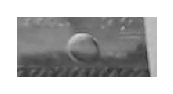
\includegraphics[width=\textwidth]{Figures/SizeFinder1.eps}
            \caption{Raw Image}
            \label{fig:size:1}
        \end{subfigure}
        ~ %add desired spacing between images, e. g. ~, \quad, \qquad, \hfill etc. 
          %(or a blank line to force the subfigure onto a new line)
        \begin{subfigure}[b]{0.3\textwidth}
            
\includegraphics[width=\textwidth]{Figures/SizeFinder2.eps}
            \caption{Background Subtraction}
            \label{fig:size:2}
        \end{subfigure}
        ~ %add desired spacing between images, e. g. ~, \quad, \qquad, \hfill etc. 
        %(or a blank line to force the subfigure onto a new line)
        \begin{subfigure}[b]{0.3\textwidth}
            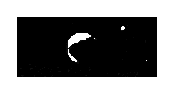
\includegraphics[width=\textwidth]{Figures/SizeFinder3.eps}
            \caption{Top Hat}
            \label{fig:size:3}
        \end{subfigure}
    
        \begin{subfigure}[b]{0.3\textwidth}
            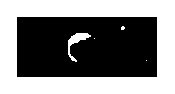
\includegraphics[width=\textwidth]{Figures/SizeFinder4.eps}
            \caption{Binarise}
            \label{fig:size:4}
        \end{subfigure}
        ~ %add desired spacing between images, e. g. ~, \quad, \qquad, \hfill etc. 
          %(or a blank line to force the subfigure onto a new line)
        \begin{subfigure}[b]{0.3\textwidth}
            
\includegraphics[width=\textwidth]{Figures/SizeFinder5.eps}
            \caption{Convex Hull}
            \label{fig:size:5}
        \end{subfigure}
        ~ %add desired spacing between images, e. g. ~, \quad, \qquad, \hfill etc. 
        %(or a blank line to force the subfigure onto a new line)
        \begin{subfigure}[b]{0.3\textwidth}
            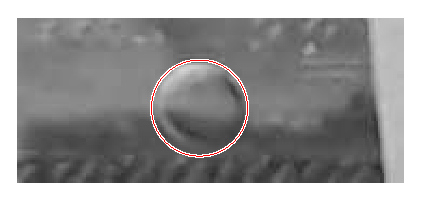
\includegraphics[width=\textwidth]{Figures/SizeFinder6.eps}
            \caption{Detected Circle}
            \label{fig:size:6}
        \end{subfigure}
        \caption{Figure }\label{fig:size}
    \end{figure}
    
    There are a few drawbacks to this algorithm. For one, it is highly sensitive to noise, meaning that if the oil is cloudy then it will fail. The top-hat filter is also semi-manual, and must be tweaked for different droplet colours/transparencies. It also struggles with droplets with a radius below 0.3mm. Finally, it also relies on our assumption that the droplets are perfectly spherical, which is not completely true.\\
    
    The error produced by this algorithm was also considered. As we will discuss later, determination of droplet radius only requires knowledge of the width of a bounding box drawn around the sphere. As such, the diameter of 20 droplets of approximately fixed size was determined both by hand and by algorithm to the nearest pixel. 100\% of the droplets were detected by the algorithm to within 4 pixels in diameter. Given that the diameter of the 2mm thick channel corresponded to approximately 80 pixels, it can be estimated that the boundary of a droplet can be calculated to within 5\% error. \\
    
    This error is largely due to the pixel-level precision and small number of pixels taken up by the droplet. As the droplets produced for the experiment were typically 25 pixels in radius, they only took up 2000 of the 2073600 pixels in a 1920x1080 image. If the camera had a lower focal length it could be positioned far closer to the droplet, allowing droplets to take up more than 0.1\% of the pixels of the image. A higher resolution camera would also increase the accuracy of boundary detection. \\
    
    With knowledge of the perimeter of the droplet, a bounding box could be placed around each droplet, pixels converted to mm, and Equation \ref{eq:radii} used to determine the droplet radius.
    
    From this point, the motor could be re-engaged, and the photodiode probed.

    \subsection{Determining Values}

    

    


\section{Results}

\section{Discussion}
% -----------
% REFERENCES
% -----------
\newpage

\bibliographystyle{unsrtnat}
\bibliography{references}
    

% -----------
% FIN
% -----------
\end{document}